 % DPF 09 talk on strangeness in nucleon

\documentclass[10pt]{beamer}
\usefonttheme{professionalfonts} % using non standard fonts for beamer
\usefonttheme{serif} % default family is serif
\usepackage{amsmath}
\usepackage{ulem}
\usepackage{hyperref}
\usepackage{array}
\usepackage{mathtools}
%\documentclass[12pt]{beamerthemeSam.sty}
\usepackage{epsf}
%\usepackage{pstricks}
%\usepackage[orientation=portrait,size=A4]{beamerposter}
\geometry{paperwidth=160mm,paperheight=120mm}
%DT favorite definitions
\def\LL{\left\langle}	% left angle bracket
\def\RR{\right\rangle}	% right angle bracket
\def\LP{\left(}		% left parenthesis
\def\RP{\right)}	% right parenthesis
\def\LB{\left\{}	% left curly bracket
\def\RB{\right\}}	% right curly bracket
\def\PAR#1#2{ {{\partial #1}\over{\partial #2}} }
\def\PARTWO#1#2{ {{\partial^2 #1}\over{\partial #2}^2} }
\def\PARTWOMIX#1#2#3{ {{\partial^2 #1}\over{\partial #2 \partial #3}} }

\def\rightpartial{{\overrightarrow\partial}}
\def\leftpartial{{\overleftarrow\partial}}
\def\diffpartial{\buildrel\leftrightarrow\over\partial}

\def\BI{\begin{itemize}}
\def\EI{\end{itemize}}
\def\BE{\begin{displaymath}}
\def\EE{\end{displaymath}}
\def\BEA{\begin{eqnarray*}}
\def\EEA{\end{eqnarray*}}
\def\BNEA{\begin{eqnarray}}
\def\ENEA{\end{eqnarray}}
\def\EL{\nonumber\\}
\def\BS{\bigskip}
\def\BC{\begin{center}}
\def\EC{\end{center}}
\def\BCC{\begin{columns}}
\def\ECC{\end{columns}}
\def\HC{\column{0.5\textwidth}}

\newcommand{\etal}{{\it et al.}}
\newcommand{\gbeta}{6/g^2}
\newcommand{\la}[1]{\label{#1}}
\newcommand{\ie}{{\em i.e.\ }}
\newcommand{\eg}{{\em e.\,g.\ }}
\newcommand{\cf}{cf.\ }
\newcommand{\etc}{etc.\ }
\newcommand{\atantwo}{{\rm atan2}}
\newcommand{\Tr}{{\rm Tr}}
\newcommand{\dt}{\Delta t}
\newcommand{\op}{{\cal O}}
\newcommand{\msbar}{{\overline{\rm MS}}}
\def\chpt{\raise0.4ex\hbox{$\chi$}PT}
\def\schpt{S\raise0.4ex\hbox{$\chi$}PT}
\def\MeV{{\rm Me\!V}}
\def\GeV{{\rm Ge\!V}}

%AB: my color definitions
%\definecolor{mygarnet}{rgb}{0.445,0.184,0.215}
%\definecolor{mygold}{rgb}{0.848,0.848,0.098}
%\definecolor{myg2g}{rgb}{0.647,0.316,0.157}
\definecolor{abtitlecolor}{rgb}{0.0,0.255,0.494}
\definecolor{absecondarycolor}{rgb}{0.0,0.416,0.804}
\definecolor{abprimarycolor}{rgb}{1.0,0.686,0.0}
\definecolor{Red}           {cmyk}{0,1,1,0}
\definecolor{Grey}           {cmyk}{.7,.7,.7,0}
\definecolor{Lg}           {cmyk}{.4,.4,.4,0}
\definecolor{Blue}          {cmyk}{1,1,0,0}
\definecolor{Green}         {cmyk}{1,0,1,0}
\definecolor{Brown}         {cmyk}{0,0.81,1,0.60}
\definecolor{Black}         {cmyk}{0,0,0,1}
\definecolor{A}{rgb}{0.8,0.0,0.0}
\definecolor{B}{rgb}{0.0,0.6,0.0}
\definecolor{C}{rgb}{0.6,0.6,0.0}
\definecolor{D}{rgb}{0.0,0.0,0.5}
\definecolor{E}{rgb}{0.4,0.4,0.4}


\usetheme{Madrid}


%AB: redefinition of beamer colors
%\setbeamercolor{palette tertiary}{fg=white,bg=mygarnet}
%\setbeamercolor{palette secondary}{fg=white,bg=myg2g}
%\setbeamercolor{palette primary}{fg=black,bg=mygold}
\setbeamercolor{title}{fg=abtitlecolor}
\setbeamercolor{frametitle}{fg=abtitlecolor}
\setbeamercolor{palette tertiary}{fg=white,bg=abtitlecolor}
\setbeamercolor{palette secondary}{fg=white,bg=absecondarycolor}
\setbeamercolor{palette primary}{fg=black,bg=abprimarycolor}
\setbeamercolor{structure}{fg=abtitlecolor}

\setbeamerfont{section in toc}{series=\bfseries}

%AB: remove navigation icons
\beamertemplatenavigationsymbolsempty
\title{
  \textbf {Motion with constant acceleration}\\
%\centerline{}
%\centering
%\vspace{-0.0in}
%\includegraphics[width=0.3\textwidth]{propvalues_0093.pdf}
%\vspace{-0.3in}\\
%\label{intrograph}
}

\author[W. Freeman] {Physics 211\\Syracuse University\\Walter Freeman}

\date{\today}

\begin{document}

\frame{\titlepage}

\frame{\frametitle{\textbf{The beginning: Free fall}}
\large
\begin{center}
My purpose is to set forth a very new science dealing with a very ancient subject.
There is, in nature, perhaps nothing older than motion,
concerning which the books written by philosophers are neither few nor small
nevertheless I have discovered by experiment some properties of it which are worth
knowing and which have not hitherto been either observed or demonstrated....

\bigskip

So far as I know, no one has yet pointed out that the distances traversed, during equal intervals of time, by a body falling from rest,
stand to one another {\bf in the same ratio as the odd numbers beginning with unity.}
\bigskip
\end{center}
\bigskip
--Galileo Galilei, {\it Dialogues and Mathematical Demonstrations Concerning Two New Sciences}, 1638 (translated into English by some old dead guy)
}

\frame{
	
	\centerline{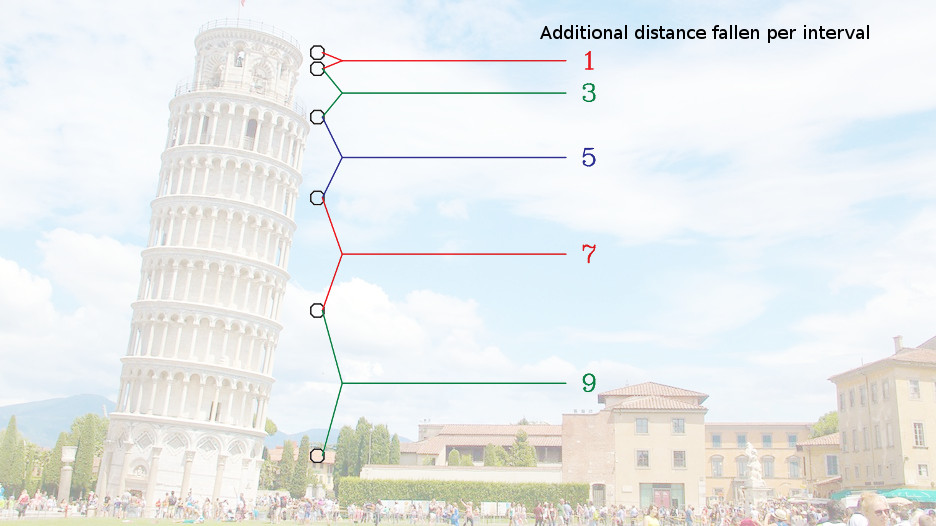
\includegraphics[width=0.9\textwidth]{pisa.jpg}}

}

\frame{\frametitle{\textbf{The beginning: Free fall}}
	\large
	\begin{center}
		I have discovered something new about something very old -- motion.
		Philosophers have written piles of thicc books about it for centuries. 
		But by doing {\it experiments}
		I've learned something they've never figured out.
		
		\bigskip
		
		None of them have figured out that a falling object travels one unit of distance, then three,
		then five, then seven, etc., in equal amounts of time.
		\bigskip
		
	\end{center}
	\bigskip
	--Galileo Galilei, {\it Dialogues and Mathematical Demonstrations Concerning Two New Sciences}, 1638 (in modern English)
}

\frame{\frametitle{\textbf{Empiricism}}
	
	\large
	
	
	The highest authority in science is what we measure.
	
	\BS
	
	If we're seeking truth about nature, the starting point {\it must be} what we see.
	
	\BS
	
	Galileo made this observation about falling objects. He {\it didn't} know why.
	
	\BS\BS\pause
	
	Our job for today:
	
	\BI
	\item Come up with a {\color{Red} model} that might explain falling
	\item Use mathematics to explore the things that our model {\color{Green}predicts}
	\BI
	\item Does our model predict Galileo's observation?
	\EI
	\item See what else our model could also explain besides falling objects
	\EI	
}


\frame{\frametitle{\textbf{Reminders:}}
\Large
\begin{itemize}
\item Webpage: \url{https://walterfreeman.github.io/phy211/}
\BI
\large
\item Syllabus, homework, etc. are all there
\EI
\item Homework 0 is a brief survey including about your math skills
\item Homework 1 will be posted today and will be due next Thursday or Friday in recitation
\EI
}

\frame{\frametitle{\textbf{``Ask a Physicist''}}
\Large There are a lot of cool things in physics that go beyond mechanics.

\bigskip
\bigskip
\bigskip

\large

If you've got questions you'd like me to address, send them in and I'll answer them!

\normalsize
\BI
\item What are gravity waves?
\item Is there a smallest distance in the universe? {\it (This is my research actually!)}
\item How is physics used in medicine? Or computer design? Or environmental science? Or the military?
\item{What's the Large Hadron Collider for?}
\item{How does a touchscreen work?}
\item{How do 3D movies work?}
\item{What is the Higgs boson?}
\item{How is physics used in video games?}
\item{How does a nuclear reactor work?}
\item How do we simulate physics using computers?
\item{How does a supercomputer work (and do this faster)?}
\EI
}

\frame{\frametitle{\textbf{Homework tips}}
\centerline{\Large Your first ``real'' homework assignment is due next Friday.}

\bigskip
\bigskip

\large
\BI
\item{Make use of words, pictures, and algebra (not just algebra!) in your reasoning}
\item{We're interested in how you think, not just the answer -- you must explain what you're doing}
\item{Physical values need to be given with units (``4 meters'', not ``4'')}
\item{Leave variables in until the very end}
\item{Paper is cheap -- don't cramp yourself!}
\pause
\bigskip
\item{Ask for help -- early and often}
\BI
\item{Email: wafreema@syr.edu}
\item{Discord server}
\item{Office hours}
\item{The Physics Clinic}
\item{Recitations}
\pause
\item{In class!}
\EI
\EI
}
%
%\frame{\frametitle{\textbf{The course webpage}}
%\large
%\BI
%\item{All notes, etc., will be posted on the course website (not Blackboard)}
%\item{I will also post course announcements there}
%\item{The syllabus is posted there}
%\EI
%
%\BS\BS
%
%
%}

\frame{\frametitle{\textbf{Office hours}}
\Large
In the Physics Clinic:
\BI
\item{Tuesdays: 2:00-4:00 PM}
\item{Fridays: 9:00 AM-11:00 AM (may change)}
\item Other times announced (if homework is due Friday, I may hold Thursday office hours)
\EI

or by appointment.  
\bigskip
\bigskip

Outside these times you might find me in the Clinic or in my office in room 215.
}

\frame{\frametitle{\textbf{The beginning: describing motion (1-D)}}
\large
Recall that at first, we are only concerned with describing motion.

\bigskip

\BI
\large
\item{Most fundamental question: ``where is the object I'm talking about?''}
\item{Quantify position using a ``number line'' marked in meters:}
\BI
\normalsize
\item{Choose one position to be the origin (``zero'') -- anywhere will do}
\item{Choose one direction to be positive}
\item{Measure everything relative to that}
\item{Can measure in any convenient units: centimeters, meters, kilometers...}
\EI

\bigskip

\item{You're used to this already, perhaps:}
\BI
\normalsize
\item{Mile markers on highways}
\item{Yard lines in American football}
\EI
\EI
}

\frame{\frametitle{\textbf{The beginning: Free fall}}
\centerline{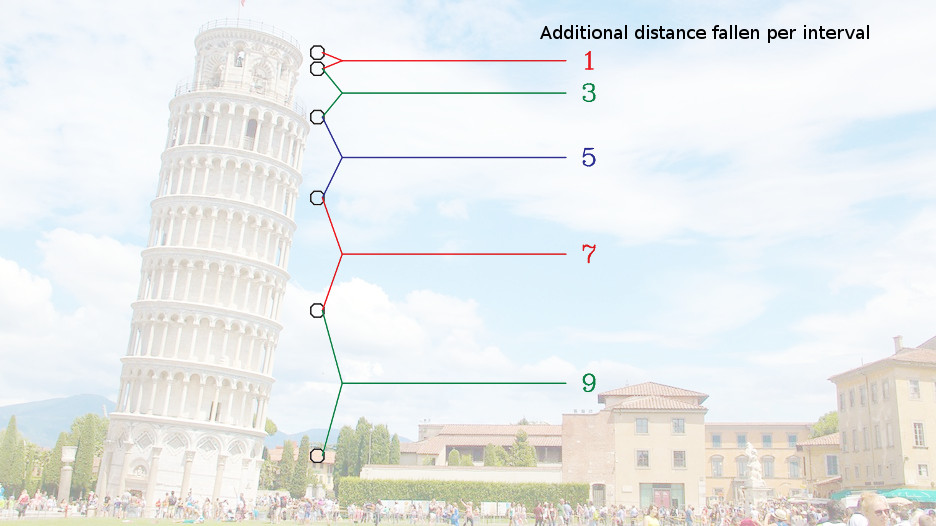
\includegraphics[width=0.8\textwidth]{pisa.jpg}}

\begin{center}
\Large Galileo observed this, but can we explain it?
\end{center}
}



\frame{\frametitle{\textbf{Equations of motion}}
\large
Complete description of motion: ``Where is my object at each point in time?''

\bigskip

This corresponds to a mathematical function. Two ways to represent these. Suppose I drop
a ball off a building, putting the origin at the ground and calling ``up'' the positive direction:

\bigskip
\bigskip

\begin{columns}
\column{0.5\textwidth}
\centerline {\color{Red}\Large Graphical representation}
\column{0.5\textwidth}
\centerline{\color{Blue} \Large Algebraic representation}
\end{columns}

\bigskip

\begin{columns}
\column{0.5\textwidth}

\centerline{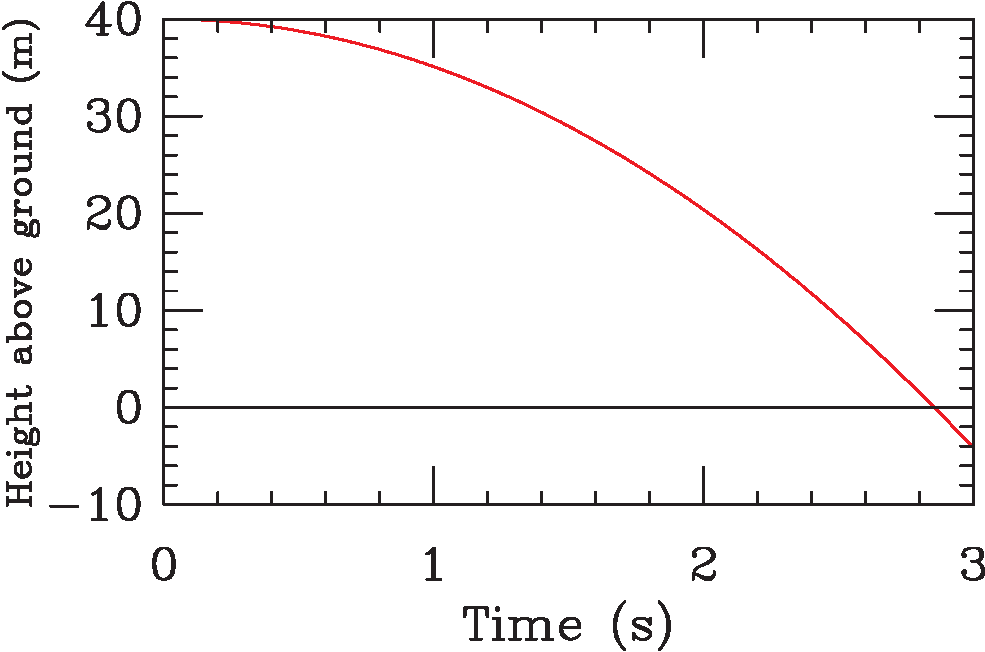
\includegraphics[width=0.7\textwidth]{falling-crop.pdf}}

\column{0.5\textwidth}
\color{Blue}
$$y(t) = (40 \,{\mathrm m}) - C t^2$$ \\
(C is some number; we'll learn what it is in a bit)

\end{columns}

\bigskip

\centerline{Both let us answer questions like ``When does the object hit the ground?''}

\bigskip

\begin{columns}
\column{0.5\textwidth}
\centerline {\color{Red}\large $\rightarrow$ ... the curve's x-intercept}
\column{0.5\textwidth}
\centerline{\color{Blue} \large $\rightarrow$ ... when $y(t)=0$}
\end{columns}

}

\frame{\frametitle{\textbf{Velocity: how fast position changes}}
\large
The slope of the position vs. time curve has a special significance. Here's one with a constant slope:

\medskip

\centerline{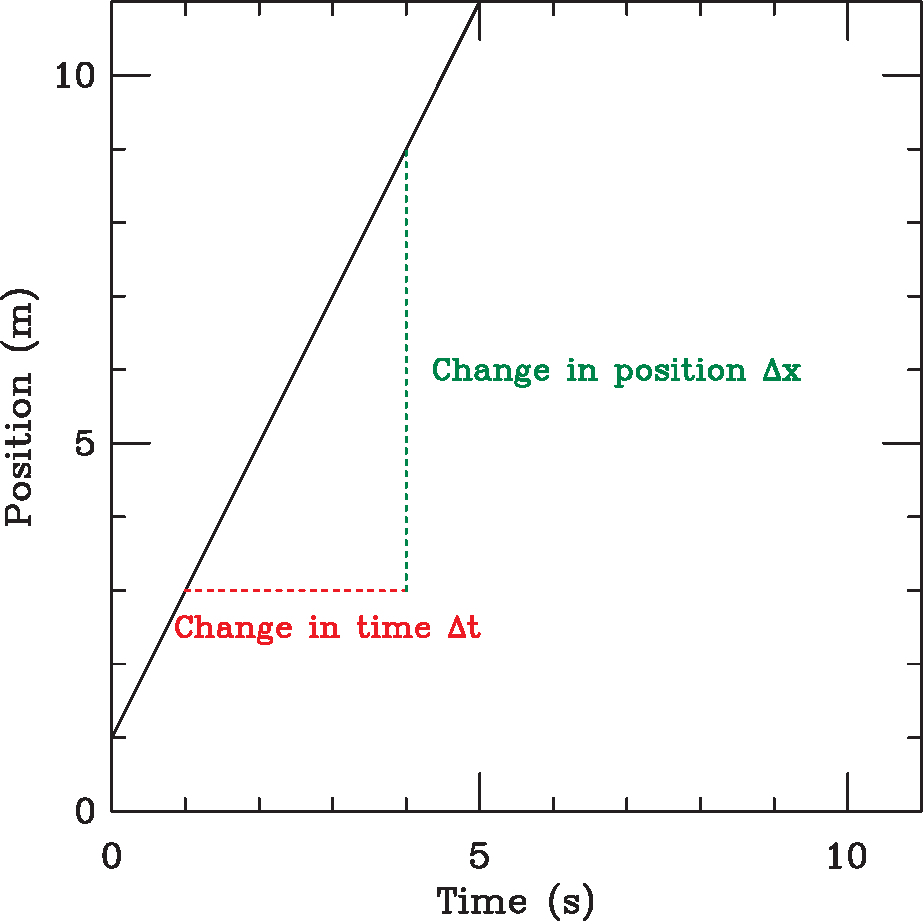
\includegraphics[width=0.4\textwidth]{constant-v-crop.pdf}}

\bigskip

\pause

Slope is $\frac{{\rm rise}}{{\rm run}}$ = $\frac{\Delta x}{\Delta t}$ = $\frac{2\,\rm m}{1 \, \rm s}$ = 2 meters per second (positive;
it could well be negative!)

\bigskip \pause

{\color{Red} $\rightarrow$ The slope here -- change in position over change in time -- is the {\bf velocity}!} Note that it can be
positive or negative, depending on which way the object moves.

}


\frame{\frametitle{\textbf{Constant-velocity motion: connecting graphs to algebra}}
\large
If an object moves with constant velocity, its position vs. time graph is a line:

\medskip

\centerline{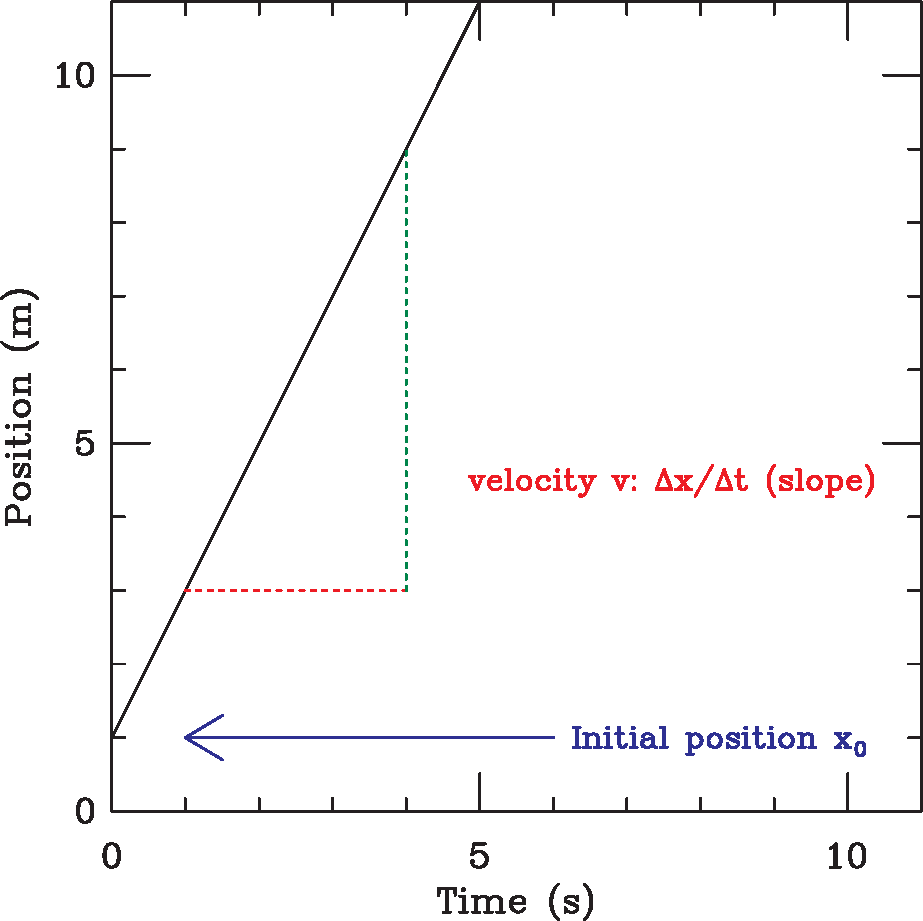
\includegraphics[width=0.4\textwidth]{constant-v-2-crop.pdf}}

We know the equation of a straight line is is $x = mt + b$ (using $t$ and $x$ as our axes).

\BI
\item{$m$ is the slope, which we identified as the velocity}
\item{$b$ is the vertical intercept, which we recognize as the value of $x$ when $t=0$}
\EI

We can thus change the variable names to be more descriptive:

\bigskip

\centerline{\Large{{\color{Red} $x(t) = vt + x_0$} (constant-velocity motion)}}

}

\frame{\frametitle{\textbf{Going from ``equations of motion'' to answers}}

\large

{\color{Red}$x(t) = vt + x_0$} is called an {\it equation of motion}; in this case, it is valid for constant-velocity motion.

\medskip

It gives you the same information as a position vs. time graph, but in algebraic form.

\bigskip
\bigskip

\normalsize

To solve real problems, we need to be able to translate physical questions into algebraic statements:
\bigskip
\bigskip

\BI
\item{``If a car starts at milepost 30 and drives at 50 mph, where is it an hour later?''}
\pause
\BI
\item{Using $x(t) = x_0 + vt$, with $x_0=30\, {\rm mi}$ and $v = 50 \frac{\rm mi}{\rm hr}$, calculate $x$ at $t=1\, {\rm hr}$}
\EI
\EI
}

\frame{\frametitle{\textbf{Asking the right questions}}

\large
``I drop an object from a height $h$. When does it hit the ground?'' How do I
do this? (Take $x_0=h$ and upward to be positive.)

\BS

Remember, we want to ask a question in terms of our physical variables. This question 
has the form:

\BS
\Large
``What is \rule{1in}{0.55mm} when \rule{1in}{0.55mm} equals \rule{1in}{0.55mm}?''

\BS
\large
Fill in the blanks.

\Large
\BS

\color{A}A: $v$, $x$, 0 \\
\color{B}B: $t$, $x$, h \\
\color{C}C: $x$, $t$, 0 \\
\color{D}D: $t$, $x$, 0 \\
\color{E}E: $x$, $v$, 0 \\
}

\frame{\frametitle{\textbf{Asking the right questions}}
\large
``At what location do two moving objects meet?''

\BS
\Large
\color{A}A: ``At what time does $x_1 = x_2$?'' \\
\color{B}B: ``At what time does $v_1 = v_2$?'' \\
\color{C}C: ``What is $x_1$ at the time when $x_1 = x_2$?'' \\
\color{D}D: ``What is $x_1$ when $t_1 = t_2$?'' \\

}


\frame{\frametitle{\textbf{Velocity, acceleration, and calculus}}
\Large
Constant-velocity motion: $x(t) = x_0 + vt$

\bigskip

\normalsize

\BI

\item{Came from looking at the equation of a line}
\item{We can understand this in a different framework, too:}

\bigskip

\item{\Large Velocity is the {\color{Red} rate of change} of position}
\BI
\item{Graphical representation: Velocity is the slope of the position vs. time graph}
\item{Mathematical language: Velocity is the {\color{Red} derivative} of position}
\EI
\EI

\bigskip
\bigskip

\Large

We know we need to know about acceleration (``F=ma'') -- what is it?

\bigskip
\BI
\item{Acceleration is the {\color{Red} rate of change} of velocity}
\EI
}


\frame{\frametitle{\textbf{Position, velocity, and acceleration}}
\begin{columns}
\column{0.125\textwidth}
\centerline{\Large Position}
\column{0.2\textwidth}
\small
{\color{Red}
\centerline{(take the derivative)}
\centerline{take the rate of change of}
\centerline{$\xrightarrow{\makebox[\textwidth]{}}$}}
\column{0.125\textwidth}
\centerline{\Large Velocity}
\pause
\column{0.2\textwidth}
\small
{\color{Red}
\centerline{(take the derivative)}
\centerline{take the rate of change of}
\centerline{$\xrightarrow{\makebox[\textwidth]{}}$}}
\column{0.15\textwidth}
\centerline{\Large Acceleration}
\end{columns}
}

\frame{\frametitle{\textbf{Kinematics: how does acceleration affect movement?}}
\Large
Newton's law $a = F/m$ tells us that {\it acceleration} -- the second derivative of position -- is what results from forces.\\

\bigskip
\bigskip
\bigskip
\pause
\begin{center}{\color{D} \bf All freely falling objects have \\a constant acceleration downward.}
\bigskip
\bigskip

This value is so important we give it a letter: $g = 9.8$ $\rm m/\rm s^2$.

\small
\bigskip\bigskip\pause

(You can approximate this as $g = 10 \rm m/\rm s^2$ unless you need high precision.)

\end{center}
}


\frame{\frametitle{\textbf{Some calculus}}
\begin{center}
If velocity is the rate of change of position, \\
why is the area under the $v$ vs. $t$ curve equal to displacement?
\end{center}

\centerline{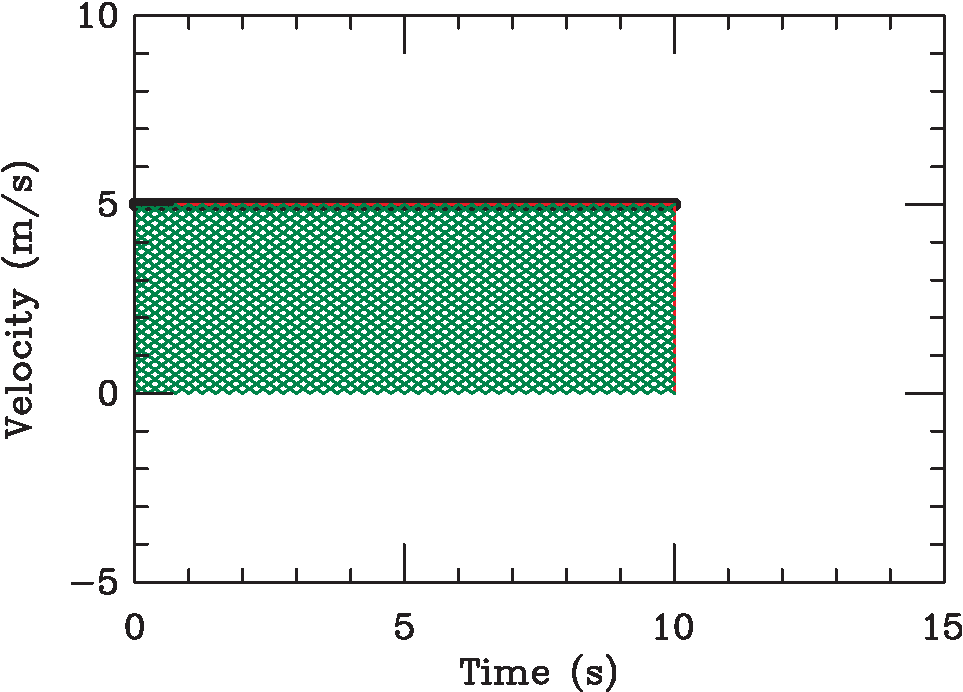
\includegraphics[width=0.7\textwidth]{integral-constant-crop.pdf}}

\bigskip

\centerline{\large We know $\Delta s = vt$. What is that here? What's the area of the shaded region?}

}

\frame{\frametitle{\textbf{Some calculus}}

\centerline{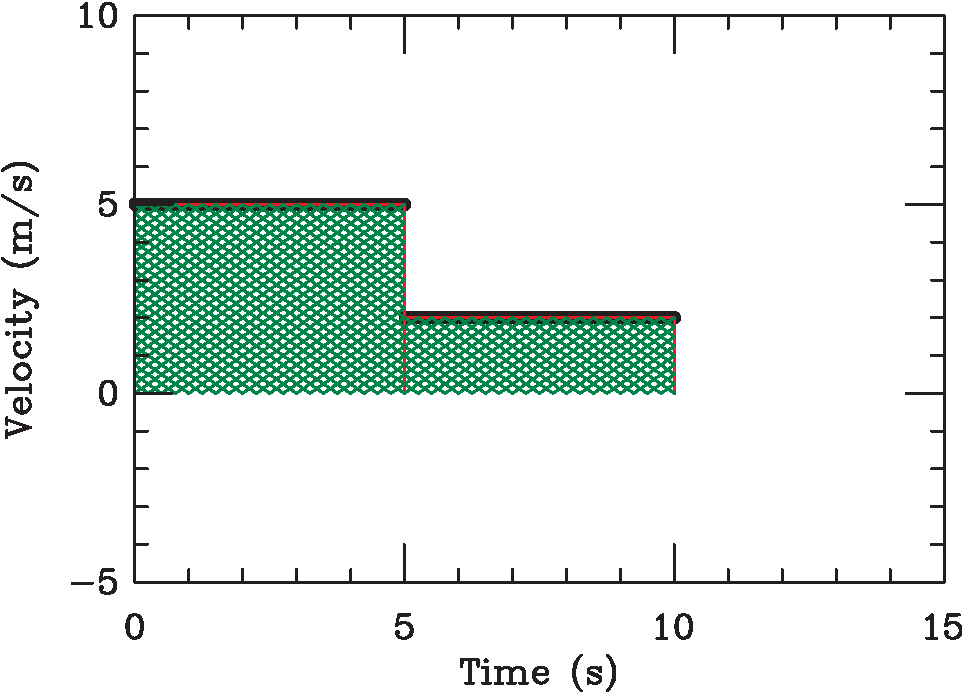
\includegraphics[width=0.6\textwidth]{integral-two-crop.pdf}}

\bigskip
\bigskip
\bigskip

\centerline{\large Now what is $\Delta s$? What is the area of the shaded region?}

}

\frame{

\Huge

What's the area of the shaded region?

\bigskip\bigskip

\color{A}A: 25 m \\
\color{B}B: 50 m \\
\color{C}C: 35 m \\
\color{D}D: 45 m \\

}


\frame{\frametitle{\textbf{A calculus review}}

\BC

What if the velocity is more complicated?

\EC


\centerline{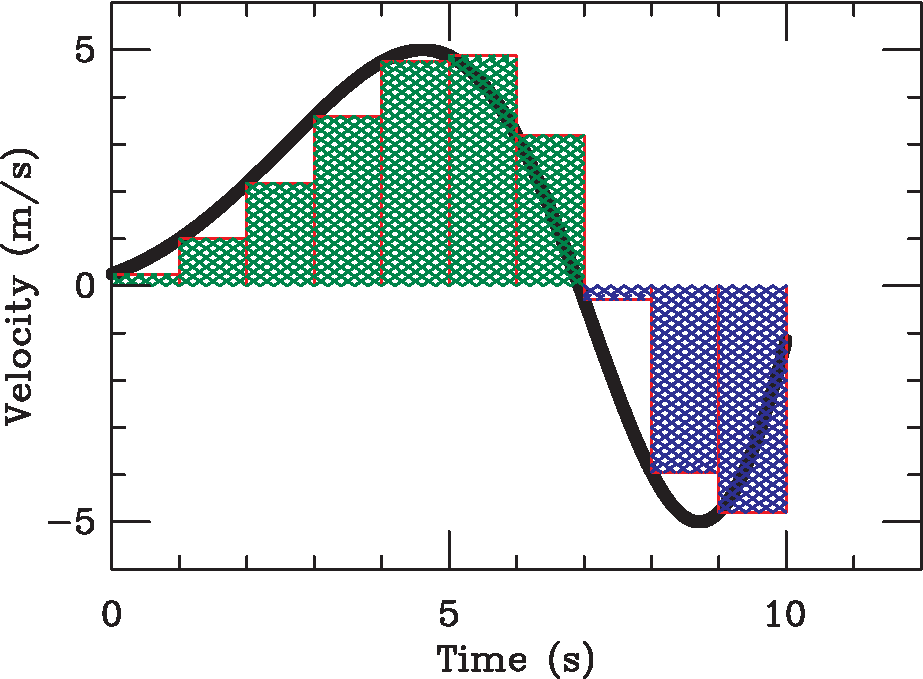
\includegraphics[width=0.6\textwidth]{integral-curve-coarse-crop.pdf}}

\bigskip
\bigskip
\bigskip

\centerline{\large Does this work? How do we fix it?}

}
\frame{\frametitle{\textbf{A calculus review}}

\centerline{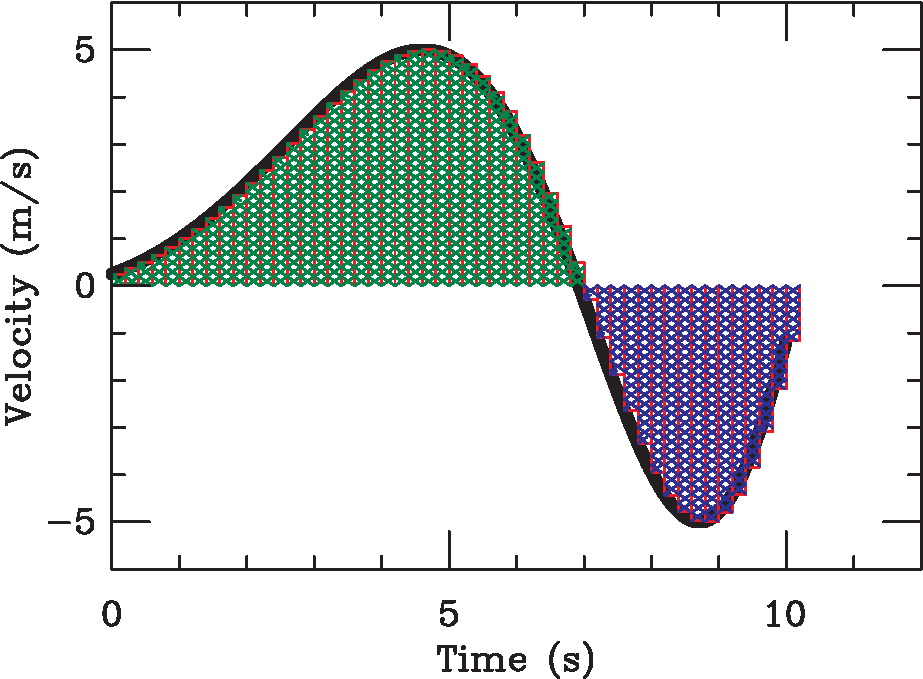
\includegraphics[width=0.6\textwidth]{integral-curve-fine-crop.pdf}}

\bigskip
\bigskip

\centerline{\large The area between the $t$-axis and the velocity curve is the distance traveled.}
\centerline{\large \color{Grey} (The area below the $t$-axis counts negative: ``the thing is going backwards''}
\bigskip
\centerline{\large In calculus notation: $\int v(t)\, dt = \Delta x = x(t) - x_0$}

}


\frame{\frametitle{\textbf{Position, velocity, and acceleration}}
\begin{columns}
\column{0.125\textwidth}
\centerline{\Large Position}
\column{0.2\textwidth}
\small
{\color{Red}
\centerline{(take the derivative of)}
\centerline{take the rate of change of}
\centerline{$\xrightarrow{\makebox[\textwidth]{}}$}}
{\color{Green}
\color{Green}\centerline{$\xleftarrow{\makebox[\textwidth]{}}$}}
\color{Green}\centerline{take the area under the curve of}
\color{Green}\centerline{(take the integral of)}
\column{0.125\textwidth}
\centerline{\Large Velocity}
\pause
\column{0.2\textwidth}
\small
{\color{Red}
\centerline{(derivative of)}
\centerline{rate of change of}
\centerline{$\xrightarrow{\makebox[\textwidth]{}}$}}
{\color{Green}
\color{Green}\centerline{$\xleftarrow{\makebox[\textwidth]{}}$}}
\color{Green}\centerline{take the area under the curve of}
\color{Green}\centerline{(take the integral of)}
\column{0.15\textwidth}
\centerline{\Large Acceleration}
\end{columns}
}

\frame{\frametitle{\textbf{Constant acceleration}}
Particularly interesting situation:
\BI
\item{Free fall (as you saw)}
\item{Any time the force is constant: $F = ma \rightarrow a = F/m$...}
\EI
\bigskip
\pause
Plan of attack:
\BI
\item{We know what the acceleration curve looks like (it's flat). How do we get the velocity curve?}
\pause
\item{\color{A} Figure out the area under the acceleration curve to get the velocity curve}
\pause

\item{\color{B} Figure out the area under the velocity curve to get the position curve}
\EI
\pause
\bigskip
\bigskip
\bigskip
\bigskip
Remember the area under the curve of (velocity, acceleration) just gives the {\it change in} (position, velocity) -- {\it i.e.} initial minus final.

\bigskip
\bigskip

\bf We'll start by assuming $x_0$ and $v_0$ are zero -- \rm that is, we're dropping something from rest.
}

\frame{\frametitle{\textbf{Constant acceleration}}
\centerline{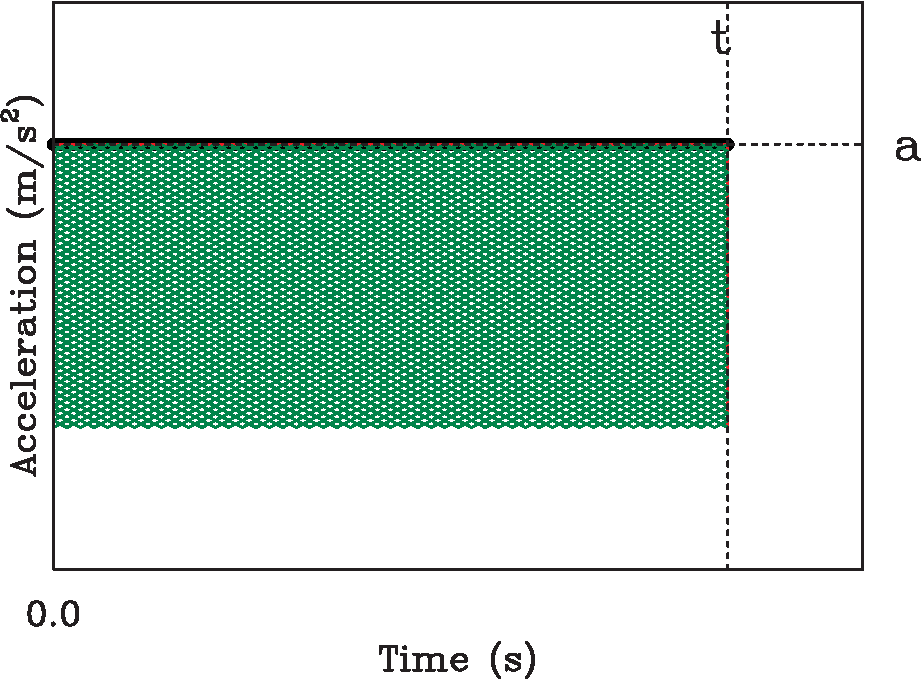
\includegraphics[width=0.6\textwidth]{area-under-a-crop.pdf}}

\bigskip


What's the area under the curve out to time $t$, which gives the change in the velocity -- $\Delta v=v(t) - v_0$?

\BS
\Large
\BCC
\HC
\color{A}A: $\Delta v = at$\\
\color{C}C: $\Delta v = \frac{1}{2}at^2$\\
\HC
\color{B}B: $\Delta v = at + v_0$\\
\color{D}D: $\Delta v = a$\\
\ECC

}


\frame{\frametitle{\textbf{Constant acceleration}}
\centerline{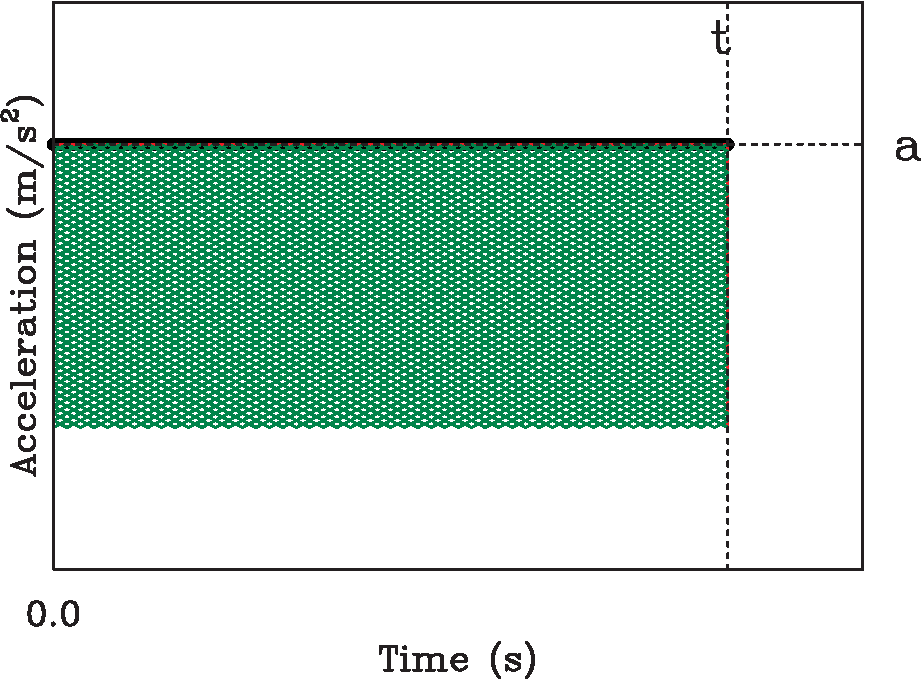
\includegraphics[width=0.6\textwidth]{area-under-a-crop.pdf}}

\bigskip


What's the area under the curve out to time $t$, which gives the change in the velocity -- $\Delta v=v(t) - v_0$?

\pause

\bigskip
\bigskip

\centerline{\Large $\Delta v$, the change in velocity, is $v(t) - v_0 = at$, so {\color{Red}$v(t) = at + v_0$}}
}

\frame{\frametitle{\textbf{Same thing again to get position}}
\centerline{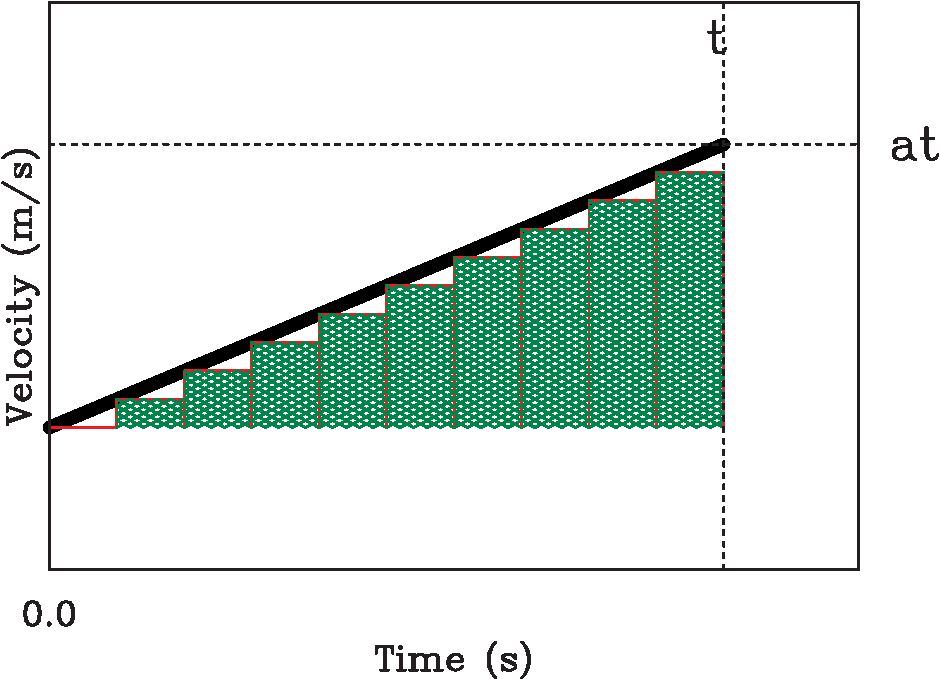
\includegraphics[width=0.6\textwidth]{area-under-v-crop.pdf}}

\bigskip


Now the area under the velocity curve gives the change in position: $\Delta x=x(t) - x_0$.
What is that?
\BS
\Large
\BCC
\HC
\color{A}A: $\Delta x = at$\\
\color{C}C: $\Delta x = \frac{1}{2}at^2$\\
\HC
\color{B}B: $\Delta x = vt$\\
\color{D}D: $\Delta x = v$
\ECC


\pause

\bigskip

\centerline{\Large $x(t) - x_0 = \frac{1}{2}at^2$, thus $x(t) = \frac{1}{2}at + x_0$}
}

\frame{\frametitle{\textbf{Now if $v_0$ is not zero...}}
\centerline{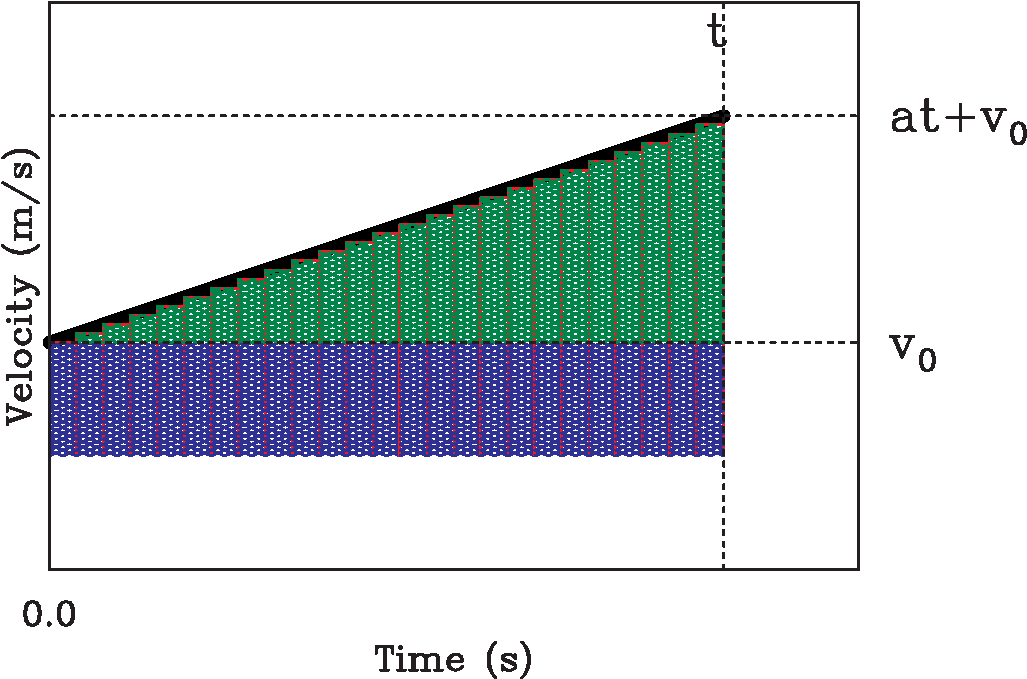
\includegraphics[width=0.6\textwidth]{area-under-v-full-crop.pdf}}

\bigskip

\pause
 \color{D}Area under blue part: $v_0 t$\\
\color{B} Area under green part: $\frac{1}{2} at^2$\\

\color{Black}Total change in position: $x(t) - x_0 = \color{B}\frac{1}{2}at^2 + \color{D}v_0 t$

\bigskip
\bigskip
\centerline{\Large Thus, {\color{Red}$x(t) = \color{B}\frac{1}{2}at^2 +\color{D} v_0 t \color{Red}+ x_0$}}
}

\frame{\frametitle{\textbf{For those who are familiar with calculus:}}

\begin{align*}
a(t) &= \rm{const}.\\
v(t) &= \int a\,dt &=& at + C_1 \\
x(t) &= \int v\,dt = \int (at + C_1) dt &=& \frac{1}{2}at^2 + C_1 t + C_2
\end{align*}

A little thought reveals that $C_1$ is the initial velocity $v_0$ and $C_2$ is the initial position $x_0$.\\
This gives us the things we just derived, but much more easily:


{\color{Red}
\Large
\begin{align*}
v(t) &=& at + v_0 \\
x(t) &=& \frac{1}{2}at^2 + v_0 t + x_0
\end{align*}}
}

\frame{\frametitle{\textbf{Free fall revisited}}
\centerline{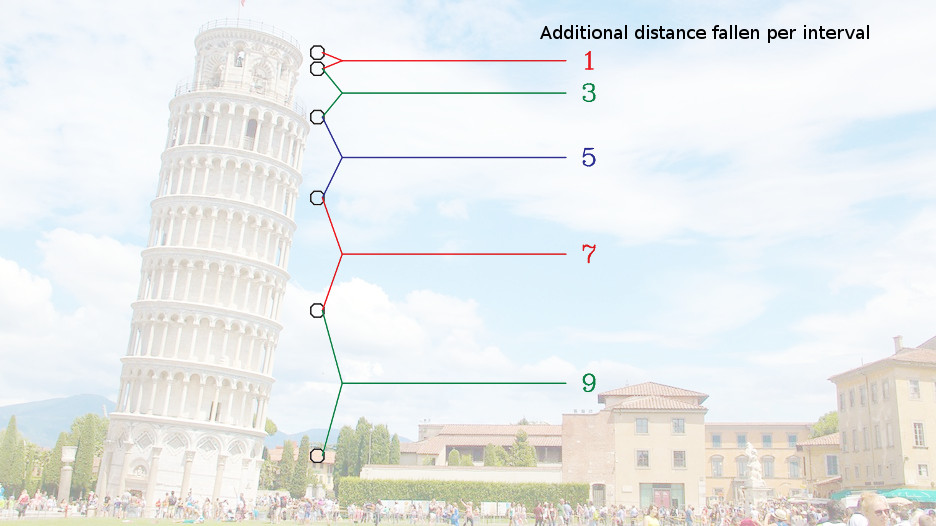
\includegraphics[width=0.8\textwidth]{pisa.jpg}}

\centerline{Adding these numbers together gives us 1, 4, 9, 16, 25...}
\centerline{The calculus above explains this: distance is proportional to {\it time squared!}}
}



\end{document}
